\section{Empirical Study Between Stack Overflow \& Russian site}
To check the relationship and difference between Stack Overflow and Russian Stack Overflow, we carry out the empirical study in two perspectives, the users and the content within each site.

\subsection{Users}

%In this part, we mainly analyse whether it is necessary to build multilingual Stack Overflow by deeply compare the user activity, the knowledge base status and the areas of focus between Stack Overflow main site and Russian Stack Overflow site. The combination of all research results can lead to a solid conclusion for the meaning of multilingual Q\&A community development. \par 

Users, especially the core users are crucial to the success of Q\&A sites~\cite{mamykina2011design}, as they play an important role in asking, answering, and helping maintain the quality of site by revising the low-quality posts.
Some users have accounts in both Stack Overflow and Russian Stack Overflow.
As two sites are both sub-sites of Stack Exchange networks, we can locate these intersection users by their Stack Exchange ID [4].
\begin{comment}
User is highly important for the analysis of a community~\cite{mamykina2011design} because the whole knowledge base is the achievement of all users during a long time of accumulation. 
Users in the intersection of Stack Overflow main site user set and Russian Stack Overflow user set, who own both accounts should be considered as one of the main research subjects.
Besides, the key users who contributed much to the community are also this paper's important research subjects.  
According to the Stack Overflow policy, a user has a different user id on the specific site, while a unique account id to link these two users on the entire Stack Exchange Network [4]. 
\end{comment}
By December 8th, 2017, there are 8,123,937 users on Stack Overflow main site and 98,125 users on Russian Stack Overflow site. 
51,415 users owns both accounts at the same time, accounting for 52.4\% of the total number of the users on Russian Stack Overflow.



\subsubsection{Creation date}
\textcolor{red}{CCY: We tune-down the \textbf{migration} and avoid mentioning it in the paper.}
%Focusing on this intersection user base, the user migration can be measured by comparing their account creation dates of both site. 
Among these 51,415 intersection users, 32,288 (62.8\%) of them sign up their  Stack Overflow account first then sign up Russian Stack Overflow i.e., coming from Stack Overflow.
Those users take up 32.9\% of the population in Russian Stack Overflow, which shows the significant importance of the Stack Overflow to the Russian one.
But compared with total 8.1 million users in Stack Overflow, it takes only 0.40\%.
So even all of these users migrate from Stack Overflow to the Russian one, it is still a small influence to the main site.


On the other hand, there are also 19,125 (37.2\%) users getting accounts of Russian Stack Overflow first, and then also register Stack Overflow.
It means that to some extent, the launch of Russian Stack Overflow also help 
grow users of the main site which further reduce the potential loss of the main site.
\textcolor{red}{Find an example user who sign up RSO first, and ask/answer many questions in RSO. Then he migrate to SO to ask/answer many questions.}
 
\begin{comment}
\begin{figure}[!h]
	\centering
	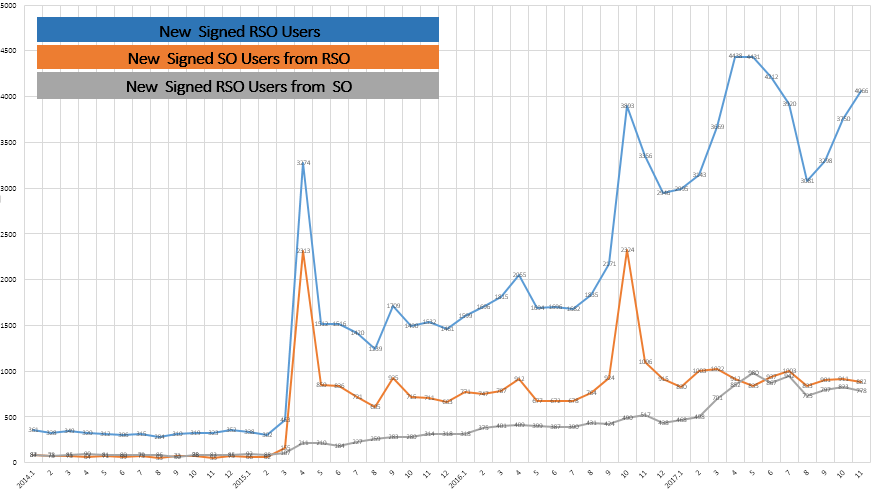
\includegraphics[width = 0.7\textwidth]{figures/userflow.png}
	\caption{The Sign Up for different sites}
	\centering
	\text{\scriptsize(SO for Stackoverflow and RSO for Russian Stackoverflow)}
	\label{fig:signup}
\end{figure} 
 
To illustrate the user migration in details, Figure~\ref{fig:signup} presents the statics of the users who sign up a Russian Stack Overflow account from Jan 1st, 2014 (the launch time of Russian Stack Overflow) to Dec. 8th, 2017. 
As shown in the figure, the new users who migrated from Stack Overflow main site 
occupy a high proportion, and also the Russian site attracts and \textcolor{red}{feedbacks a growing 
number of users ??what does this mean? not good English} to the main site with the time going by. 
In other words, the main 
site and the multilingual version both have a positive effect on the other one, which 
means both of them can \textcolor{red}{assist the development of the other ??this conclusion contradicts to that of last paragraph!}. This phenomenon means 
the development of multilingual version is helpful for the development of the main 
site.
%This phenomenon means the development of multilingual version is helpful for the development of the main site.	
\end{comment}

\textbf{Summary}: Although many users in Russian Stack Overflow have Stack Overflow accounts first, such population (0.40\%) is rather minor to  Stack Overflow.

\subsubsection {Location}
To zoom in the influence of Russian Stack Overflow to the Russian users in Stack Overflow, We try to identify users in Stack Overflow who are from Russia or can speak Russian.
In Stack Overflow, users can create their own profiles by filling in their names, location, AboutMe (self introduction), GitHub link, etc.
\textcolor{red}{CCY:take a screenshot of a Russian users portfolio whose place is in Russian and aboutME contain Russian words.}
To find Russian users in Stack Overflow, we first check if the user location is in Russia.
Note that if the location is written in English, we determine that it is in Russian by  \textcolor{red}{...CCY: Please add the detail and the tool that you use for this purpose.} 
If the location contains any Russian letters, we regard the place in the Russia.
Through the location, we find \textcolor{red}{??} users who may be from Russia.
Then for other users, we further check if their AboutMe contain any Russian letters and take them (\textcolor{red}{???} users) as Russian.
Totally, we find that \textcolor{red}{???34,705} users in Stack Overflow are from Russia.
Among them, 10,699 (30.8\%) have registered Russian Stack Overflow, which shows that compared with other-country users, Russian Stack Overflow does have attractions to many Russian users in Stack Overflow. 
Note that within these 10,699 users, only 6,537 (61.1\%) users registered Stack Overflow first, while the other 4,162 (38.9\%) of them created Russian Stack Overflow first
It indicates that not only can Russian Stack Overflow attract users in Stack Overflow, but Stack Overflow can also benefit from Russian Stack Overflow.
Such phenomenon mitigates the user loss of Stack Overflow.

\textbf{Summary}:
Russian Stack Overflow does attract Russian users in Stack Overflow, but Stack Overflow also benefits the new users from Russian Stack Overflow.
 
\begin{comment}
To identity the Russian users on the Stack Overflow main site, the location information of registered users has also been analyzed. The users whose location are places in Russia (either written in English or in Russian) as well as the ones whose AboutMe sections contain Russians are marked as Russian related users, indicating their native language is probably Russian. The collected statistics is shown in Table~\ref{tab:loc}. Under this assumption, there are \textcolor{red}{34,705 Russian related users ??why not 51415 in Section 2.1.1?} registered on the Stack Overflow main site. Among these users, 10,699 (30.8\%) users have the Russian Stack Overflow account at the same time which means the rest majority of Russian users only use the main site. 
Also, within these 10,699 users, 6,537 (61.1\%) users migrated from main site to Russian site and 4,162 (38.9\%) users migrated from Russian site to main site. Most Russian related users (69.2\%) on the Stack Overflow still only have the main site account rather than migrating to the Russian Stack Overflow.  
\begin{table}[h!]
	\centering
	\caption{Location and AboutMe information analysis (users count among 8,123,937 main site users)}
	\label{tab:tablex}
	\begin{tabular}{lrr}
		Filter & \#Location Info. & \#AboutMe Info.\\
		\hline
		contain non-englsih word & 111,006  &  35,000\\
		contain Russian Letter & 9,858 &  2,079\\
		contain Russian Places & 24,468 & 1,718\\
	\end{tabular}
    \begin{tabular}{lr}
    	\hline
    	Total Russian related users: & 34,705\\
    	Russian related users with RSO account: & 10,699\\
    \end{tabular}
	\label{tab:loc}
\end{table}	
\end{comment}
 

\subsubsection{Reputation Score}
In Stack Overflow, users can get reputation scores by getting upvotes on their questions, answer and comments. Reputation score represents how much contribution a user has made,how much the community trusts you and how well the peer users think about your work in the community.
The higher score user gets, the high reputation he/she earns. Thus, the more reputation a user earned, the higher level of activity the user has. So it is a qualified value to measure the active users by calculating this variable. Figure~\ref{fig:reputationDistribution} shows the statics of reputation of users in Russian Stack Overflow by segregating all 98,125 users into 3 groups. Local users (in Blue) on Russian Stack Overflow who do not own an account of the main site are 46,712 (47.6\%). The migrated users from Main site (in Red) are 32,288 (32.9\%) and the migrated users from Russian site (in Green) are 19,125 (19.5\%). Figure~\ref{fig:reputationDistribution} shows the different reputation scores distribution among these three group users.

Considering the Reputation Bonus Policy that a starting plus 100 reputation bonus 
to users who already have a 200+ account of any site belongs to Stack Exchange [5], the 32,288  users who migrated from the main site reasonably have a large number of 
the reputation level of 100 to 200. However, despite the local user, the remains are 
the user who owns both account of the main site and Russian version. Under the 
circumstance that the number of migrants is almost \textcolor{red}{2 times ??32288/19125 about 1.7 times, not 2. In a technical paper, has to be very specific} of that of the 19,125 users 
who sign up Russian version account first, \textcolor{red}{the later contributes somehow an equal 
number of active users ??how can we tell this from Fig. 3?}.

To some degree, the reputation reveals that multilingual communities \textcolor{red}{are not dominated 
by a large number of external users even the later has an overwhelming advantage 
on the user amount ??do not understand how this conclusion can be reached from the reputation distribution analysis?}, which means that multilingual communities are relatively 
independent in the respect of user contribution in the community development process.


%In Stack Exchange, once a user get more than 200 reputation points, he will get site %association bonus i.e., 100 points on each site in Stack Exchange, as Stack Exchange regards %that user as trusted [5]
%~\cite{https://stackoverflow.com/help/whats-reputation}.
%Therefore, we regard users with 200+ reputation score in Russian Stack Overflow as its core %users.
%Considering the Reputation Bonus Policy that a starting plus 100 reputation bonus to users who already have a 200+ account of any site belongs to Stack Exchange [5], the 29,609 users who migrated from the main site reasonably have a large number of the reputation level of 100 to 200. 

%However, there are 384,304 core users in Stack Overflow, and only 885 of them migrate to %Russian Stack Overflow.
%Figure~\ref{fig:reputationDistribution} displays the detailed reputation score distribution, %and most migrated user actually lay in the range between 100 to 200.
%That is because the core user in Stack Overflow can get 100 reputation points once they join %Russian Stack Overflow, but they are not counted as active in the new site as they are not %active to get another 100 points.  
%Among 3,390 core users, only 885 (28.24\%) of them come from Stack Overflow.
%It demonstrates again that Stack Overflow is merely hurt by the launch of Russian Stack %Overflow, and Russian Stack Overflow is rather independent.
%However, despite the local user, the remains are the user who owns both account of the main site and Russian version. 
\begin{figure}
	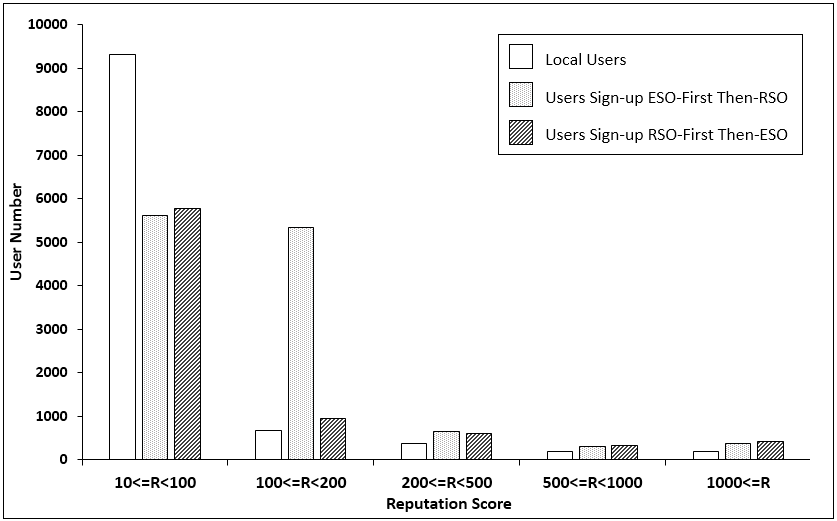
\includegraphics[width = 0.49\textwidth]{figures/reputation.png}
	\caption{The reputation distribution in Russian Stack Overflow}
	\label{fig:reputationDistribution}
\end{figure} 

%\textcolor{red}{Actually, it is wrong to define migration as in this paper, because although some people come from Stack Overflow, they can only be regarded as migrated only if they are active in Russian Stack Overflow, but not active in the main site any more. But we do not have enough time to revise it.}

%\textbf{Summary:} 28.24\% core users in Russian Stack Overflow migrate from Stack Overflow.
%Under the circumstance that the number of migrants is almost 2 times of that of the 16,155 users who sign up Russian version account first, the later contributes somehow an equal number of active users.
%To some degree, the reputation reveals that multilingual communities are not dominated by a large number of external users even the later has an overwhelming advantage on the user amount, which means that multilingual communities are relatively independent in the respect of user contribution in the community development process.


\subsection{Content}
After exploring the users between Stack Overflow and Russian site, this empirical study further analyse the content between two sites from different aspects.

\subsubsection{Post}
In Q\&A website, users communicate with each other by asking questions and answer questions.
We regards both questions and answers as posts.
In Russian Stack Overflow, there are totally 400,185 posts, and we count how many posts are created by different users.
The results can be seen in Table~\ref{tab:postnumber}.
We can see that more that 6,201 (6.3\%) users who have created more than 10 posts have contributed to 75.9\% content of Russian Stack Overflow.
Due to their importance to the site, we regard these 6,201 users as the core users.

\begin{table}
	\centering
	\caption{Post statics}
	\label{tab:postnumber}
	\begin{tabular}{lrrrr}
		\hline
		\#User Post & \#Post & Post percentage& \#User &User percentage \\
		\hline
		P\_C$>=$2 &372,046&92.9\%&24,908&25.4\%\\
		P\_C$>=$4 &345,543&86.3\%&13,526&13.8\%\\
		P\_C$>=$6 &328,398&82.1\%&9,644&9.8\%\\
		P\_C$>=$8 &314,833&78.7\%&7,537&7.7\%\\
		P\_C$>=$10&303,604&75.9\%&6,201&6.3\%\\
		\hline
	\end{tabular}
\end{table}	

\begin{comment}
Post is the prime part in the content of a Q\&A websites since post is the rising of the question as well as the origin of the answers and comment. It is also a very suitable variable to find the active users and popular topics in the Q\&A website community. Although every user has the right to post a question and add comments, the composition of the knowledge base ought to obey \textcolor{red}{the Pareto Law, which means 20\% of the users make 80\% of the contribution ??where do you find this? any reference or support? in general, literature says power law. how can know 20\% versus 80\%?}.
 
Imagine that a post is a single unit, and millions of posts consist of the knowledge base, and each post includes maybe a lot of answers and comments in the tree structure. 
From Table 1 it is already clear that there are totally 400,185 posts for the Russian Stack Overflow, and using the unique account id to calculate the amount of post for each user on Russian Stack Overflow, the results are presented in Table~\ref{tab:postnumber}. 	



From the table, the static distribution can be easily seen. As mentioned above, with the number of a single user post sum growing, the user proportion decrease. Notice that 6,201 (6.3\%) people from the 98,125 Russian Stack Overflow users who have 10 or more posts contribute 75.9\% of the post amount. These users could be labled as ´ Core User´ in this study representing the ones who have the highest level of contribution. Again, in these 6,201 core users, 1,845 people
are local users while 4,356 people own both main site account and Russian sub-site
account at the same time. In these 4,356 users in the intersection, 1,835 people are
migrants from the Stack Overflow main site. This distribution has been shown in Figure~\ref{fig:reputationTree}.

For the \textcolor{red}{1,676 ??where is this number from? never appear above?} of Core Users who sign up the Stack Overflow account first, which also known as the migrant from the main site, they post 104,448 posts on Russian sub-site that count 26.1\% of the post amount on Russian sub-site. For the \textcolor{red}{2,521 ??where is this number from?} of Core Users who sign up the Russian sub-site account first, which also known as the migrant from the main site, they post 139,275 posts on Russian sub-site that count 34.8\% of the post amount on Russian sub-site. According to the average level, the external users do not dominate the post area. 

\end{comment}

Among these 6201 core users, 4356 of them own both Stack Overflow and Russian Stack Overflow account (seen in Fig~\ref{fig:reputationTree}). 
1835 users registered Stack Overflow first, and created 139,275 posts on Russian Stack Overflow which counts 34.8\% of all posts.
It shows that although many core users may come from Stack Overflow they do not dominate Russian Stack Overflow.
Actually most contributions come from local users in the Russian site.

\begin{figure}
	\centering
	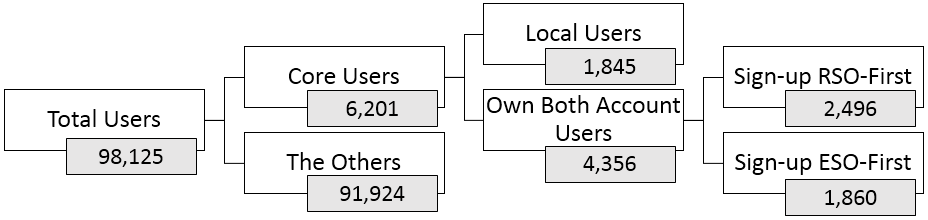
\includegraphics[width = 0.3\textwidth]{figures/usercomponent.png}
	\caption{User components on Russian Stack Overflow \textcolor{red}{CCY:Please draw this figure horizontally to save some space.}}
	\centering
	\label{fig:reputationTree}
\end{figure}

A core user owning both accounts in two sites and registering Stack Overflow first does not necessarily demonstrates that he migrate from Stack Overflow to the Russian one.
To locate users who migrate from Stack Overflow to the Russian one, we define the following formula: 

\textcolor{red}{CCY: This formula seems wrong. It should be that the $\#MainsitePostCountAfterRegistration/TimeLengthAfterRegistration$, so need to re-calculate it.}
\begin{equation}
	f = \frac{\#RussianPostCountAfterRegistration/TimeLengthAfterRegistration}{  \#MainsitePostCountBeforeRegistration /TimeLengthBeforeRegistration}	 
	\label{equ:active}
\end{equation}

The larger value represents the more possibility one user migrate from Stack Overflow to Russian Stack Overflow.
It means that if a core user in Russian Stack Overflow is more likely migrant if he creates fewer posts in Stack Overflow after his registration of the Russian one than that before his registration.

\begin{comment}
Moreover, for the 1,835 of Core Users who sign up the Stack Overflow account first,
according to their frequency of post activity, it can be also concluded that they are still
spending more time and concentrate on the Stack Overflow main site. The formula of
judging a migrant is Formula~\ref{equ:active}. If the f value is greater than 1, the user transferred his or her main active area to the new site.
\end{comment}

	
Assume that a reasonable range for the unchanged active level that is 0.8 to \textcolor{red}{1.2 ??why not 1?} for f, the results in Table~\ref{tab:table3} reveal that more than half of those active users from the main site tend to be more active in a multilingual sub-site. Although they are from another site, they make a lot of contribution and seem to be like using the new sub-site regularly. The conclusion of the research on post aspect is the multilingual community has a group of users as backbone so that the community is not dominated by the users from the Stack Overflow main site, but the migrants from the main site are also willing to contribute in the new community.
\begin{table}
	\scriptsize
	\centering
	\caption{Statics for the \textcolor{red}{1,676} Users who post more than 10 and from Stack Overflow main site \textcolor{red}{CCY: The statistic seem totally wrong. Please check it carefully!!!}}
	\label{tab:table3}
	\begin{tabular}{p{1.1cm}|p{1.2cm}|p{0.8cm}|p{1.6cm}|p{0.8cm}}
		\hline
		User Post count & User Amount & f $<$ 0.8 & 0.8$<=$f$<=$1.2 &f $>$ 1.2 \\
		\hline
		P\_C$>=$10 & 1,860  &707 & 120 & 1033   \\
		P\_C$>=$20 & 445  & 208 & 39 & 198\\
		P\_C$>=$50 & 228 & 134 & 18 & 76 \\
		P\_C$>=$100& 134 & 94 & 11 & 29 \\
		\hline
	\end{tabular}
\end{table}	

%\textbf{Summary:} The migrated users from Stack Overflow main site are not dominant in the Russian subsite.


\subsubsection{Tag}
A tag is a word or phrase that describes the topic of the question. 
It can represent the overall technology landscape of the site~\cite{???ChunyangKG}.
%The tag is a means of connecting experts with questions, and they will be able to answer the question by sorting questions into specific and well-designed categories. 
%Research on the tags is able to reveal a number of most hot fields and topics in the Q\&A website content. 
In Stack Overflow or the Russian one, each question can have up to five tags. 
There are 50,812 tags on Stack Overflow and 3,957 tags in the Russian one. 
Among these 3,957 tags, 821 of them contain Russian character and the other 3,136 are in English. 
To check the overlap and difference of tags between Russian Stack Overflow and Stack Overflow, we first translate Russian tags into English with Google Translate, and then \textcolor{red}{manually revise some incorrect translations ??give some typical examples of such manual corrections?} to make them identical to the main site ones.
2,560 (64.7\%) out of 3,957 tags of Russian Stack Overflow also exist on the Stack Overflow main site. 
And \textcolor{red}{56 CCY: we should tell the number of top-100 tags in RSO which are also covered in the whole SO.}of the top 100 frequent tags of Russian Stack Overflow also exist in the set of the top 100 frequent tags of Stack Overflow main site. 
\textcolor{red}{CCY: We need a tag cloud for both RSO and SO to show the overlap between them.}
As seen in Fig~\ref{fig:??}, most popular tags in the two sites are very similar which show the commonness between two sites.

Although most tags in Russian Stack Overflow also appear in Stack Overflow, but there is still some difference between them.
For example, some tags are unique in Russian Stack Overflow such as \textbf{Yandx} (the largest Russian search engine like Google) and \textbf{VKontakte} (biggest social network company like Facebook).
As these tags or service are Russian-specific, they are rarely used outside of Russia.
However, as a general global site, Stack Overflow will not include them.
Therefore, Russian Stack Overflow provide a perfect place to contain such culture-related technical Q\&A discussions.
\textcolor{red}{CCY: Go on to add some other tags which appear much more frequently in Russian than that in overall Stack Overflow.}

\begin{comment}
	%Ranking the top 10 frequent tags in several sets to show what are the most popular fields in both sites.
\begin{table}[!h]
	\scriptsize
	\centering
	\caption{Top 10 Popular Tags Ranking Statics \textcolor{red}{1) How is freq \% calculated? Need to explain in the discussion. 2) Tags only in Russian should be a separate table. They are not top-10 popular tags.}}
	\label{tab:table4}
	\begin{tabular}{|p{0.8cm}<{\centering}|p{0.55cm}<{\centering}|p{0.8cm}<{\centering}|p{0.55cm}<{\centering}|p{1.5cm}<{\centering}|p{0.55cm}<{\centering}|}
	\hline
	{\scriptsize Main site tags} & freq. (\%) &{\scriptsize Russian site tags} & freq. (\%) &{\scriptsize Tags only in Russian site} & freq. (\%) \\
	\hline
	javascript & 3.39 & php & 6.51  & bootstrap  & 0.304 \\
	\hline
	java & 3.04 & javascript& 5.83  &\bf vkontakte-api & 0.200 \\
	\hline
	c\# & 2.63 & java & 5.31 & android-sdk & 0.178 \\
	\hline
	php & 2.59 & android & 4.43 & android-fragment & 0.143 \\
	\hline    
	android & 2.38 & c\#& 3.89 & mvc & 0.139 \\
	\hline    
	jquery & 2.01 & html & 3.21 & google-maps-api &0.109 \\
	\hline    
	python & 1.87 & jquery& 2.82 & golang & 0.106 \\
	\hline    
	html & 1.59 & c++ & 2.75 & cookie & 0.105 \\
	\hline    
	c++ & 1.23 & css & 2.47  & cms & 0.102 \\
	\hline    
	ios & 1.22 & mysql & 2.08  & \bf yandex-maps-api & 0.092 \\
	\hline 
	\end{tabular}
\end{table}		
\end{comment}

\begin{table}[!h]
	\scriptsize
	\centering
	\caption{Different tags preference between two sites \textcolor{red}{why this set of tags as examples? Please tell how do you get this set of tags.}}
	\label{tab:table_tagpref}
	\begin{tabular}{|l l l l l|}
		\hline
		{\scriptsize Tags} & freq. in SO (\%) & freq. in RSO (\%) & Rank in SO & Rank in RSO \\
		\hline
		web-application & 0.047 & 0.49 & 322  & 32 \\
		\hline
		yii2 & 0.03 & 0.45 & 518  & 35 \\
		\hline
		cuda & 0.029 & 0.012 & 528 & 870 \\
		\hline
		winforms & 0.2 & 0.5 & 63 & 29 \\
		\hline    
		Unity3D & 0.08 & 0.029 & 175 & 58 \\
		\hline    
		website & 0.02 & 0.485 & 734 & 31 \\
		\hline    
		layout & 0.057 & 0.42 & 287 & 41 \\
		\hline    
		Joomla & 0.037 & 0.125 & 424 & 145 \\
		\hline    
	\end{tabular}
\end{table}	


%According to the result shown in Table~\ref{tab:table4}, it is clear that the most popular areas of two sites are very similar. Though there is some difference among the \textcolor{red}{frequency numbers of the same tag ??you mean absolute frequency number? they are not comparable as the two site are of very different scale, not just due to different preference?} due to the different preference of two sites' users. Overall, 8 of the top 10 most popular tags on Russian site are also the top 10 popular tags on the main site. This indicates that the popular area and content between two sites are highly overlapped. However, focusing on some unique tags in Russian site, it appears some tags who also own considerable frequency. For example, {\bf Yandx}, which is {\bf \foreignlanguage{russian}{Яндекс} }in Russian, is a Russian multinational technology company specializing in search engine and it is the most used search engine in Russia.{\bf []} And {\bf VKontakte}, another Russian local company, is the biggest social network company in Russia and its website, vk.com, is the most popular webstie in Russia.{\bf []} It shows that the Russian sub-site does have some specialness in the content area.

\textbf{Summary}:
According to the tag analysis, majority of tags in Russian Stack Overflow are also on the main site. Moreover, it finds that Russian site is highly overlapped with the main site on the popular tags which indicate two sites may have similar content among the popular topics. On the other hand, Russian site also has its unique tags whose related posts make an non-ignorable part of all posts. 


\subsection{Links}

Hyperlink is a good tool to recommend and refer the existing content to other users. 
%Not only links can refer the knowledge base in the same site, but also across different sub-sites, or external resources. 
%Under the site announcement of Japanese Stack Overflow, one user commented, ``''
As Stack Overflow and Russian Stack Overflow are both programming-related website, it is expected that some new questions asked in the Russian Stack Overflow may have already answered or highly related to Stack Overflow.
So there should be some mutual links between them.
In this section, we try to valid such assumptions with the analysis of existing links between them.
%In this section, we explore the relationships between Stack Overflow and Russian Stack Overflow according to their mutual hyperlinks. 

%The link amount and the direction reveal the similarity and difference between these two sites.

\noindent \fbox{\centering%
    \parbox{1.0\textwidth}{%
        \textit{``This is the world wide web and it is built on a thing called hypertext. Multiple languages? Cool, that's the "world" part. But don't forget about hypertext. Please, make sure that questions and answers can be linked easily across the different language sites. If someone asks a question in Japanese that is essentially a duplicate of an existing English question, linking the two questions will allow Japanese speakers (who might understand *some* English, or at least be able to read code snippets) to get immediate value from past answers, without waiting for new answers... ''
        }
        
        {\raggedleft --- one comment under the announcement of Japanese Stack Overflow\par}
            }%
}
\\

\begin{table}
	\caption{Links Statics \textcolor{red}{Please make sure that this statistics are totally right. In addition, the link should not contain the image links.}}
	\centering
	\small
	\label{tab:links}
	\begin{tabular}{llll}
       \hline
		Source       &\#Total links & \#Links to SO   & \#Links to RSO\\ \hline
		SO Posts     & 13,636,973    & 1,581,888 (11.6\%)      & 88 \\
		SO Comments  & 5,959,110     & 1,835,405 (30.8\%)    & 164\\
		RSO Posts    & 131,964       & 5,674  (4.3\%)        & 5,014 (3.8\%) \\
		RSO Comments & 55,471        & 4,548  (8.2\%)        & 5,658 (10.2\%) \\
       \hline
	\end{tabular}

\end{table}	

In (Russian) Stack Overflow, users are allowed to add links in their posts (both questions and answers) and comments to refer to other resources. 
We count all links in two sites and analyse the link direction within and across two sites.
The statistics of links of two sites are summarised in Table~\ref{tab:links}.
Rarely, the links in Stack Overflow direct to Russian Stack Overflow.
But in contrast, many links in Russian Stack Overflow has been referring to Stack Overflow.
For example, in Russian Stack Overflow, 4.3\% links in posts and 8.2\% links in comments are refering to Stack Overflow.
However, compared with Russian Stack Overflow, we can see that 11.6\% links in posts and 30.8\% links in comments are from itself in Stack Overflow.
\textcolor{red}{CCY: this argument is a little far-fectched, how to say that more naturally in the paper?}
Such a large difference of link source leads to two potential reasons: 1)There is not enough overlap content between two sites; 2) Stack Overflow may be under-referenced in Russian Stack Overflow.
But as both Stack Overflow and the Russian one own millions of questions and answers, it is difficult for us to observe to determine which reason accounts for the relative small proportion of links to Stack Overflow.
Therefore, we propose a cross-site retrieval method to assist our observation and validate the reason mentioned above.
 
\begin{comment} 
Although the number seems not very big, but it is even more than the in-site links (3.8\%).
Furthermore, the links (8.2\%) in Russian Stack Overflow post to Stack Overflow is also comparable to itself (10.2\%).
Considering the links can be referring to any site in the world, this percentage is rather high, and it indicates the significant influence of Stack Overflow to the Russian one.
According to our observation, we find that the reason is like the posts in Figure~\ref{fig:answerExample}.
Some questions asked in Russian Stack Overflow are already asked or even answered in the main site, and the only difference is that it is expressed in Russian instead of English.	

But apart from existing mutual links between two sites, we find that some posts in Russian Stack Overflow are also highly related to posts in Stack Overflow, and such relationship has not been explicitly annotated by links.
For example, Fig~\ref{fig:??} shows two questions in two site respectively, and they express the same meaning, but the link to this earlier Stack Oveflow post does not appear in the later Russian post.\textcolor{red}{CCY: please find an example pair that one question in Stack Overflow is almost the same to one question in Stack Overflow, but such link has not been annotated.}
We conclude two reasons for the miss of such links.
First, the language gap between two sites limit the users in Russian Stack Overflow to find related English question.
Second, as Stack Overflow is larger and larger (tens of millions of questions and answers), it is difficult for users, especially non-native speakers to spot related questions in such a big corpus.
Therefore, a tool for finding related posts in two sites is highly needed to help bridge the gap between two sites, and also save time by avoiding duplicate efforts.
\end{comment}


\subsubsection{Method for cross-site retrieval}
\textcolor{red}{Please draw a flow chart for the overall method}
Fig~\ref{fig:flowChart} displays the overall method to retrieve related questions in Stack Overflow.
The overall method can be separated into two parts i.e., prepare the data from  Stack Overflow as the database, and then formulate the Russian Stack Overflow question as query for retrieval.
So we first preprocess the content of Stack Overflow

Given one question in Russian Stack overflow, we first translate its title and content description into English with Google Translate~\cite{??}.
After that, we extract keywords from the translation

\subsubsection{Manual validation of cross-site reference\\}


\begin{comment}
As we can see, the number of links that Russian users used to refer posts on Stack Overflow main site is smaller than the number of links that they used to refer posts on the Russian sub-site. Apparently, the results of the links show that Russian Stack Overflow sub-site is relatively independent because it owns a considerable proportion of links referring the existing post in its own knowledge base. The Russian sub-site does not completely depend on Stack Overflow main site, as the Russian users are not always referring the existing posts on main site. However, in some ways the Russian Stack Overflow sub-site has a non-negligible demand of knowledge reference from the main site. So the content of these two sites are not totally same and not totally different, especially the Russian subsite has its necessity of existence.	content...
\end{comment}

\textbf{Summary}: 
Many hyperlinks in Russian Stack Overflow come from the main site which shows the Stack Overflow is an important information resource for the Russian one.
But it is not enough, and more links are further needed to bridge the gap between two sites.

\begin{comment}
\subsection{Conclusion}
The above empirical comparison between two sites shows that Russian Stack Overflow owns many unique features which are not included by the main Stack Overflow, no matter its users or Russian-specific content.
Such difference demonstrate that the existence of the multi-lingual Stack Overflow is meaningful and useful to some specific users.
Furthermore, the multi-lingual deviation does not significantly undermine the knowledge accumulation or user participation of the main site.
\end{comment}